% CVPR 2022 Paper Template
% based on the CVPR template provided by Ming-Ming Cheng (https://github.com/MCG-NKU/CVPR_Template)
% modified and extended by Stefan Roth (stefan.roth@NOSPAMtu-darmstadt.de)

\documentclass[10pt,twocolumn,letterpaper]{article}

%%%%%%%%% PAPER TYPE  - PLEASE UPDATE FOR FINAL VERSION
\usepackage[review]{cvpr}      % To produce the REVIEW version
% \usepackage{cvpr}              % To produce the CAMERA-READY version
%\usepackage[pagenumbers]{cvpr} % To force page numbers, e.g. for an arXiv version

% Include other packages here, before hyperref.
\usepackage{graphicx}
\usepackage{amsmath}
\usepackage{amssymb}
\usepackage{booktabs}


% It is strongly recommended to use hyperref, especially for the review version.
% hyperref with option pagebackref eases the reviewers' job.
% Please disable hyperref *only* if you encounter grave issues, e.g. with the
% file validation for the camera-ready version.
%
% If you comment hyperref and then uncomment it, you should delete
% ReviewTempalte.aux before re-running LaTeX.
% (Or just hit 'q' on the first LaTeX run, let it finish, and you
%  should be clear).
\usepackage[pagebackref,breaklinks,colorlinks]{hyperref}


% Support for easy cross-referencing
\usepackage[capitalize]{cleveref}
\crefname{section}{Sec.}{Secs.}
\Crefname{section}{Section}{Sections}
\Crefname{table}{Table}{Tables}
\crefname{table}{Tab.}{Tabs.}


%%%%%%%%% PAPER ID  - PLEASE UPDATE
\def\cvprPaperID{*****} % *** Enter the CVPR Paper ID here
\def\confName{CVPR}
\def\confYear{2022}

\newcommand{\AJ}[1]{{\color{red}{[Andrej: #1]}}}

\begin{document}

%%%%%%%%% TITLE - PLEASE UPDATE
\title{Self-Supervised Transfer Learning From 2D Images to 3D Point Clouds}

\author{Andrej Janda\\
University of Toronto Institute for Aerospace Studies\\
Institution1 address\\
{\tt\small andrej.janda@robotics.utias.utoronto.ca}
% For a paper whose authors are all at the same institution,
% omit the following lines up until the closing ``}''.
% Additional authors and addresses can be added with ``\and'',
% just like the second author.
% To save space, use either the email address or home page, not both
\and
Jonathan Kelly\\
University of Toronto Institute for Aerospace Studies\\
First line of institution2 address\\
{\tt\small jonathan.kelly@robotics.utias.utoronto.ca}
}
\maketitle

%%%%%%%%% ABSTRACT
\begin{abstract}
    We show that previous work \cite{xie2020pointcontrast} on self-supervised contrastive learning of 3D point clouds relies on extrapolating points in the scene and not from learning noise as was claimed in the original paper. We then investigate if using 2D pre-trained features transfered to 3D can do as well as fully supervised learning.
\end{abstract}

%%%%%%%%% BODY TEXT
\section{Introduction}
\label{sec:intro}

% Write topic sentences and go from there
Segmentation of indoor 3D scenes has the potential to allow robots to navigate and interact with complicated industrial environments, such as warehouses and production facilities. Although robots already play a limited role in these facilities, understanding their surroundings would give them much greater autonomy. For instance, through segmentation, an accurate up-to-date digital twin of a physical area can be maintained for the purposes of inventory management, item retrieval, and item routing. Advances in segmentation of 3D point clouds \cite{choy20194d} has made this closer to reality.

Alternatively, segmentation of 2D images has come a long way. But it does not give us information about the 3D world and so we are left with projecting these predictions into 3D. This was the approach taken by \cite{} but has recently been overtaken by methods operating purely in 3D.

In contrast to 2D images which are bountiful, easy to collect and annotate, 3D scenes are hard to collect, not very abundant and notoriously hard to annotate. Collecting 3D scenes requires a user to physically scan different environments with complicated sensors (\eg stereo cameras, Lidar) and estimate the mapping between measurements to generate a completed scene. Since not everyone has access to these sensors, they cannot be easily scrapped off of the web. Still, the hardest component is annotation which requires users to manipulate 3D scenes and select only those points that belong to a particular object. This motivates us to look for ways of avoiding the annotation process and leverage un-labeled 3D data instead.

It is common practice in image tasks to use a model that was pre-trained in a supervised way on a larger but different dataset. However, recent works have been exploring the use of self-supervised objectives without labels in 2D image classification and found that they can greatly improve downstream accuracy, even matching fully supervised training \cite{}.

Recently, works such as \cite{xie2020pointcontrast} have shown that these methods also work with 3D data. Similar to 2D methods they use a contrastive loss objective where the goal is to learn distinguishing features between different datapoints and their respective augmentations.

These algorithms work exclusively with point clouds but throw away the corresponding images of the scene which provide a rich and dense source in extra information that can be used in downstream training. This paper investigates how this extra data modality can be leveraged. Additionally, it investigates the properties of an existing 3D pre-training algorithm.

This paper has the following contributions.

\begin{itemize}
    \item Demonstrates that previous work in 3D \cite{xie2020pointcontrast} works by learning to extrapolate 3D scenes. When purely learning improved features on fully-overlapping regions the performance gain disapears.
    \item Provide a 2D feature extractor and pre-training algorithm. Demonstrate that these features can improve 2D segmentation.
    \item Transfer learned 2D features onto a 3D model
\end{itemize}

\section{Related Work}
\label{sec:relatedWork}


\textbf{Sparse 3D convolutions.} Talk about submanifold networks, Minkowski Engine, etc

\textbf{Contrastive Learning.} Talk about SimCLR, BOYL, etc. Then talk about PointContrast.

\textbf{Knowledge Distilation} Need to read up on this


\section{Self-Supervised Contrastive learning}
\label{sec:contrastiveLearning}

The goal of self-supervised transfer learning is to learn from unlabeled data using a self-supervised objective which in turn initializes a model's backbone. The initialization is meant to improve performance of downstream tasks. Specifically, contrastive learning uses an objective function that encourages the outputs of a model on similar datapoints to be close together while keeping those of dissimilar datapoints to be far apart, in some metric space.

Defining what datapoints are similar and dissimilar depends on the pretext task. Image colorization for example defines color pixels and their grayscale equivalent as similar and all other pixels as dissimilar. In this work, we adopt the instance discrimination task as in \cite{} whereby each input individually is taken to belong to its own class.

We follow the formulation from \cite{le-khac_contrastive_2020}. Given a sampled point $\mathbf{x}$, positive points are sampled according to a positive distribution $\mathbf{x}^{+} \sim p^{+}( \cdot | \mathbf{x})$ which is commonly defined as a set of transformations $t$ of the original point. Often, positive pairs are derived by applying two different augmentations to the input point, $\mathbf{x}^{+} = t_{1}(\mathbf{x}), \, \mathbf{x} = t_{2}(\mathbf{x})$. Conversely, negative points are sampled according to $\mathbf{x}^{-} \sim p^{-}( \cdot | \mathbf{x})$ which in the context of an instance discriminative task means that they are taken as any other point not derived from the input point, regardless of its augmentation.

This point is fed through an encoder $e()$ to get feature $\mathbf{v} = e(\mathbf{x}), \mathbf{v} \in \mathbb{R}^d$. This encoder is the backbone of the model we are trying to initialize. The embedding is subsequently passed through a decoder $h()$ to generate a normalized latent representation $\mathbf{z}=h(\mathbf{v})$ with $\{\mathbf{z} \, | \, \mathbf{z} \in \mathbb{R}^{m}, \lVert \mathbf{z} \lVert^{2} = 1\}$  and where $m \leq d$. Once pretrained, only the encoder parameters are retained as the initialized backbone.

As for the objective function, we adopt an InfoNCE (Info Noise Contrastive Estimation) loss. It computes a negative log probability of an embedding's similarity to the embedding of its corresponding positive sample. This is conditioned by the similarity of that embedding to all the negative embeddings. It is defined as:
\begin{equation}
    \mathcal{L}_{i} = -\log \frac{\exp(\mathbf{z}_{i} \cdot \mathbf{z}^{+}_{i} / \tau)}{\exp(\mathbf{z}_{i} \cdot \mathbf{z}^{+}_{i} / \tau) + \sum^{K}_{j}\exp(\mathbf{z}_{i} \cdot \mathbf{z}^{-}_{j} / \tau)}
    \label{eq:contrastive_loss}
\end{equation}

Where $\tau \in (0,1]$ and represents the temperature parameter that controls the smoothness of the latent representations. $K$ is a hyperparameter that represents the number of negative embeddings to sample. Similarity between features is computed as the dot product.

\section{Feature Extraction}
\label{sec:featureExtraction}

This section goes through the types of backbones used as well as how features are extracted from 2D images and transferred to a 3D model.

\AJ{Need a picture depicting the pipeline}

\subsection{Extracting 2D features}
\label{sec:method:features2d}

We follow the ResUNet architecture from Godard \etal \cite{godard2019Digging}, which proved hugely successful in self-supervised monocular depth estimation. Its backbone consists of a ResNet34 with weights that were pretrained on ImageNet. Instead of estimating depth however, our decoder computes a 16 dimensional feature vector for each pixel in the input image.

Images are selected from the desired pre-training dataset. Positive samples are generated by randomly cropping the image, and then applying the following transformations: random horizontal flip, random gray-scale, gaussian blur and color jitter.

Only pixels found in the overlap of the two crops are used in the objective function. Corresponding pixels are taken as positive samples while all others, including from other images in a batch are taken as negatives.

This is then passed through the loss function described in \ref{eq:contrastive_loss}.

\AJ{Add figure of what your feature extractor looks like}

\AJ{Need to review how I do this in the code, I think I use a projector left over from BYOL}

\subsection{Feature projection}
\label{sec:featureProjection}

Here we leverage that images are a projection of 3D space. We assume that from a given viewpoint we have both an image as well as a depth or range scan, which is often the case when capturing raw data. Unlike in \cite{xie2020pointcontrast}, we don't require a pose linking adjacent frames making our method applicable to more use cases.

The two modalities can be mapped by projecting the point cloud into the color image using a standard pinhole camera model as defined below \cite{?}:

\begin{equation}
    \begin{bmatrix}
        u \\
        v \\
        1
    \end{bmatrix} = \frac{1}{z}
    \begin{bmatrix}
        f_u & 0   & c_u & 0 \\
        0   & f_v & c_v & 0 \\
        0   & 0   & 0   & 1 \\
    \end{bmatrix}
    \begin{bmatrix}
        x \\
        y \\
        z \\
        1 \\
    \end{bmatrix}
    \label{eq:pinhole}
\end{equation}

\AJ{Is this equation necessary or is this considered common knowledge}

Where $f$ represents focal length, $c$ the center offset, $u,v$ the pixels of an image and $x,y,z$ the 3D coordinates of the input point.

In the case of stereo cameras, this step is unnecessary as the mapping comes directly from the depth image. Note that its important to have the viewpoints of the 2D and 3D sensors be as close together as possible. This is exactly true for stereo cameras, but not guaranteed when using different sensors for each modality. Its important because occluded points can falsely be mapped to a pixel even though they are not directly visible in the image. Note also that using scans as opposed to any point cloud is also a limitation of \cite{xie2020pointcontrast}.

If the viewpoints are slightly off or the point cloud is a reconstruction from multiple scans, hidden points can be removed using the algorithm from Katz \etal \cite{katz2007Direct}.

After passing in the image through the model, the output is a scaled version of the original image. To complete the mapping, we can either take the feature with the closest feature pixel or interpolate the features using bi-linear interpolation. We will show an analysis of these two methods in section \ref{sec:results}

\AJ{Do I need to give the equation for Bi-linear interpolation or is this also considered basic knowledge}

\subsection{Feature Transfer}
\label{sec:featureTransfer}

Our last step, after generating 2D features and mapping them to 3D points is to train our 3D model to emulate our pre-trained features. We accomplish this using the same contrastive loss from \ref{eq:contrastive_loss} but with input embeddings $\mathbf{z}_i$ coming from the features of the 3D points and its positive and negative embeddings $\mathbf{z}_i^{+},\mathbf{z}_i^{-}$ coming from the corresponding 2D feature.

Only the required transformations are applied to the 2D image. These being: resizing, square cropping and colour normalization. Point cloud coordinates are transformed with a random horizontal flip and random rotation around the $z$ axis while their colors are transformed using autocontrast, translation and jitter.

We use the same 3D model as in \cite{xie2020pointcontrast}. For downstream tasks, the final $1\times1$ convolution is thrown away as the decoder.

\AJ{Need to look at not using a projection head in 3D model.}

\begin{table*}[t!]
    \centering
    \resizebox{\textwidth}{!}{
        \begin{tabular}{ c | c c c c c c c c c c c c c | c }
                                        & ceiling         & floor          & wall           & beam           & column         & window         & door           & table          & chair          & sofa           & bookcase       & board          & clutter        & mIOU                    \\
            \hline
            Scratch                     & 90.34           & \textbf{96.84} & 80.63          & 0              & 25.5           & 56.95          & 62.93          & 75.14          & 86.21          & 65.77          & 72.12          & 76.91          & 56.4           & 65.06                   \\
            Supervised                  & \textbf{91.81}  & 96.74          & \textbf{84.11} & \textbf{0.21}  & \textbf{34.68} & \textbf{57.64} & \textbf{81.53} & \textbf{77.63} & \textbf{89.82} & \textbf{85.76} & \textbf{76.03} & \textbf{79.27} & \textbf{57.67} & \textbf{70.22} (+5.16)  \\
            \hline
            PointContrast               & \textbf{92.118} & \textbf{96.93} & 82.2           & 0              & 24.94          & 53.78          & \textbf{76.91} & 75.94          & 87.93          & 70.27          & 71.2           & \textbf{77.76} & 56.36          & \textbf{66.641} (+1.58) \\
            PointContrast - theirs      & 91.97           & 96.67          & 82.4           & 0              & 17.84          & 56.49          & 75.39          & \textbf{77.63} & 87.35          & 63.3           & 73.53          & 79.55          & 58.76          & 66.22 (+1.16)           \\
            PointContrast - No Overhang & 91.624          & 96.86          & 82.02          & 0              & 29.37          & \textbf{57.5}  & 64.93          & 75.49          & 87.36          & 59.32          & 71.42          & 76.61          & 56.11          & 65.28 (+0.22)           \\
            CME \textbf{(Ours)}         & 90.8            & 96.57          & \textbf{82.52} & \textbf{0.110} & \textbf{30.94} & 56.94          & 68.71          & 75.12          & \textbf{88.48} & \textbf{71.7}  & \textbf{72.17} & 73.783         & \textbf{56.35} & 66.48 (+1.42)           \\
        \end{tabular}
    }
    \caption{S3DIS Semantic Segmentation results (mIOU)}
    \label{table:s3disResults}
\end{table*}

\begin{table*}[t!]
    \centering
    \resizebox{0.8\textwidth}{!}{
        \begin{tabular}{ c | c c c c c c c c c c | c }
                                   & beam & column        & window        & door          & table         & chair         & sofa          & bookcase      & board         & clutter       & mAP@0.5              \\
            \hline
            Scratch                & 0    & 12.8          & 61.7          & 92.0          & 51.4          & 87.3          & 62.4          & 38.5          & 87.0          & 37.1          & 53.0                 \\
            Supervised             & 0    & 26.0          & 74.3          & 84.5          & 43.3          & 87.3          & \textbf{81.8} & 37.4          & \textbf{85.4} & \textbf{41.2} & \textbf{56.2} (+3.2) \\
            \hline
            PointContrast - theirs &      & 24.7          & 67.9          & 90.7          & 43.8          & 92.0          & 72.7          & 32.3          & 85.6          & 38.0          & 54.8 (+1.8)          \\
            PointContrast          & 0    & 17.4          & 68.2          & \textbf{93.0} & 45.7          & 88.5          & 63.6          & 34.1          & 82.1          & 38.2          & 53.1 (+0.1)          \\
            CME \textbf{(Ours)}    & 0    & \textbf{35.0} & \textbf{70.0} & 83.4          & \textbf{53.9} & \textbf{88.9} & 71.7          & \textbf{42.2} & 76.1          & 36.7          & 55.8 (+2.8)          \\
        \end{tabular}
    }
    \caption{S3DIS Instance Segmentation Results (mAP@0.5)}
    \label{table:s3disInstanceSegmention}
\end{table*}

\begin{table}[t!]
    \centering

    \begin{tabular}{ c | c c c c c c}
                            & 5\%  & 10\% & 20\% & 30\% & 40\% & 100\% \\
        \hline
        Scratch             & 56.9 &      & 64.1 &      & 65.6 &       \\
        \hline
        PointContrast       &      &      &      &      &      &       \\
        CME \textbf{(Ours)} & 60.8 &      & 64.8 &      & 64.7 &       \\
    \end{tabular}

    \caption{Scannet Semantic Segmentation with Partial Data  (mIOU)}
    \label{table:scannetVaryingDataAmount}
\end{table}

% \begin{table}[t!]
%     \centering

%     \begin{tabular}{ c | c c c c c c }
%                             & 5\% & 10\% & 20\% & 30\% & 40\% & 100\% \\
%         \hline
%         Scratch             &     &      &      &      &      &       \\
%         \hline
%         PointContrast       &     &      &      &      &      &       \\
%         CME \textbf{(Ours)} &     &      &      &      &      &       \\
%     \end{tabular}

%     \caption{S3DIS Semantic Segmentation with Partial Data  (mIOU)}
%     \label{table:s3disVaryingDataAmount}
% \end{table}

\section{Experiment Results}
\label{sec:results}

This section will show (1) that the learned 2D features improve 2D segmentation performance as well as show a clear mapping to their input image when visualized. Therefore these features serve as good candidates for initializing our 3D network. (2) That the transfer of features from 2D to 3D improve performance on various 3D tasks against training from scratch. (3) That the performance of PointContrast is wholly dependant on the use of overlapping scans that allow it to extrapolate data.

\subsection{Datasets}
\label{sec:results:datasets}

Following the common practice of 3D contrastive learning \cite{xie2020pointcontrast,hou2021Exploring, zhang2021Self, jiang2021Guided}, we use the following the datasets.

\textbf{Scannet \cite{Dai2017ScanNet}:} Comprises of roughly 1600 reconstructed scans of indoor scenes captured using a stereo camera, reconstructed using a pose graph and then formed into a mesh. The scenes are mostly of individual rooms and range in the square floor size of 2 meters to 10 meters with a standard ceiling height of about 3 meters. Included in the dataset is the raw data of individual scans with their corresponding images along with the semantic and instance labels for the reconstructed scenes. It contains 20 different classes. We use the predefined train and validation split, using the validation as our test set as well as is done in previous works.

\textbf{S3DIS \cite{armeni20163D}}: Much smaller than Scannet, it comprises of only 300 scenes however their size varies quite drastically as some are of rooms and others are of entire auditoriums. The scenes were also captured using a stereo camera and are mainly of indoor office scenes. There are 13 different semantic classes and all scenes contain point level semantic and instance labels. As is commonly done \cite{xie2020pointcontrast, hou2021Exploring} we use the Area 5 split as our validation and test set.

\textbf{semanticKITTI}: Time allowing.

We use Scannet to pretrain out network as it is the largest. It shares many of the same classes and types of indoor scenes as S3DIS and so is a perfect candidate to show the use case of collecting large amounts of unlabeled data for a task and then labeling only a partial amount.

\subsection{Implementation}
\label{sec:results:implementation}

\textbf{Model:} The backbone network used is the same as that used in \cite{xie2020pointcontrast, hou2021Exploring} using the sparse convolutional library developed by \cite{choy20194d}. The backbone uses a Res16UNet34 structure with non-bottleneck blocks and a maximum feature embedding size of 256. The outputs of the model are directly used for semantic segmentation.

Instance segmentation is done using the same backbone with the head from \cite{jiang2020pointgroup}.

\textbf{Pretraining on 2D:} Batch size of 64 image pairs where for each image pair we select 4092 pixels to contrast in our loss function. The loss function uses a tau of 0.4, a learning rate of 0.01, SGD optimizer with a momentum of 0.9, dampning of 0.1 and weight decay of 0.004. We decay the learning rate according to an exponential scheduler with an exponential rate of 0.99. Trained for 20k iterations.

\textbf{Transfer:} Transfer learning is done using the scannet dataset. We use a batch size of 8 and select 2000 point-pixel combinations per datapoint. The images are only center cropped to fit into the 2D model. The 3D model uses a voxel size of 5cm. The hyperparameters are the same al those in 2D except the learning rate is set to 0.1. It is trained for 20k iterations same as pre-training on 2D.

\textbf{Downstream Tasks:} All downstream tasks are run using the pipeline and parameters from \cite{hou2021Exploring}. The only difference is that we train instead on a single GPU for 20k iterations

\subsection{Contrastive Loss in 2D}
\label{sec:results:2d}

Before transferring features into 3D, we first want to verify that the features we are transferring are useful. To do this we first visualized the features by bringing them into a 1D color space using the t-SNE \cite{maaten2008Visualizing} algorithm. the colors are put together to make an image. The visualization along with the original image can be found in figure \ref{fig:features2dvis}.

\AJ{Need to train a 2D segmentation with and without pre-training.}

\begin{figure}
    \centering
    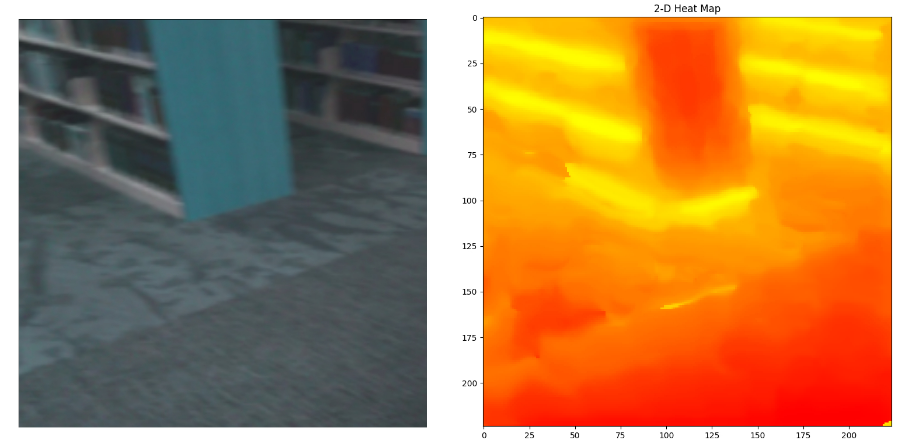
\includegraphics[width=8cm]{images/experiments/25.02.2022-image-pretrain-vis2.png}
    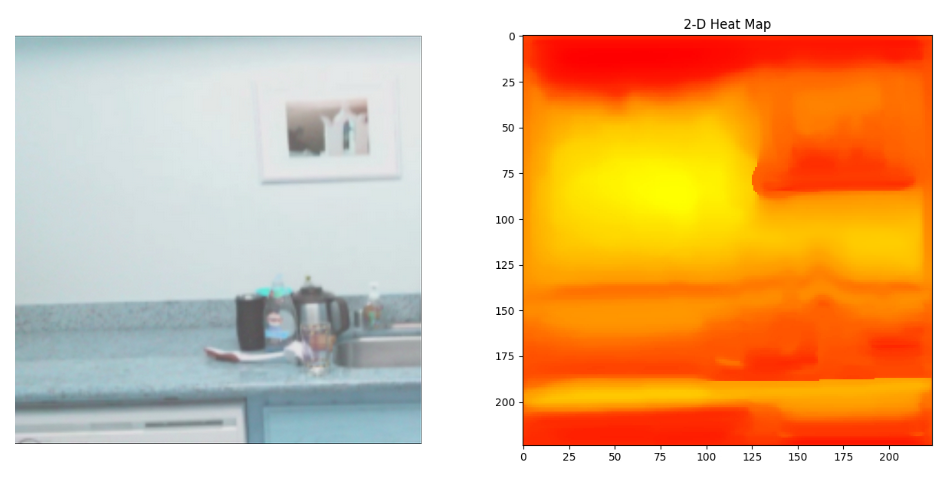
\includegraphics[width=8cm]{images/experiments/25.02.2022-image-pretrain-vis1.png}
    \caption{Visualization of features from the pre-trained 2D backbone. Images on the left are the input and right are the output.}
    \label{fig:features2dvis}
\end{figure}

\begin{figure}
    \centering
    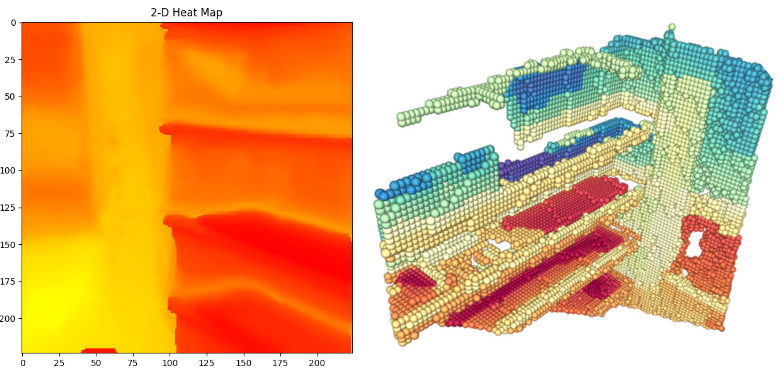
\includegraphics[width=8cm]{images/experiments/image-to-point-vis1.png}
    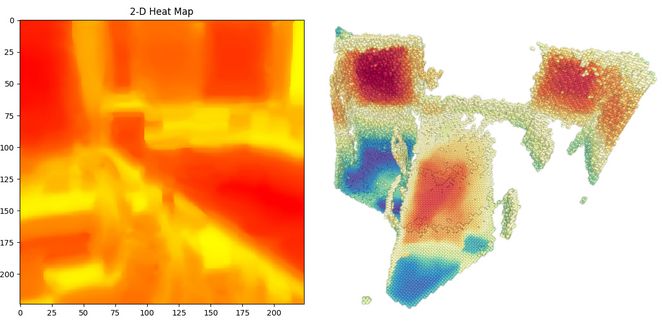
\includegraphics[width=8cm]{images/experiments/image-to-point-vis2.png}
    \caption{\textbf{left} shows features of the 2D images and \textbf{right} shows the features that were transfered to the 3D point cloud.}
    \label{fig:features2d-3dvis}
\end{figure}

\begin{figure}
    \centering
    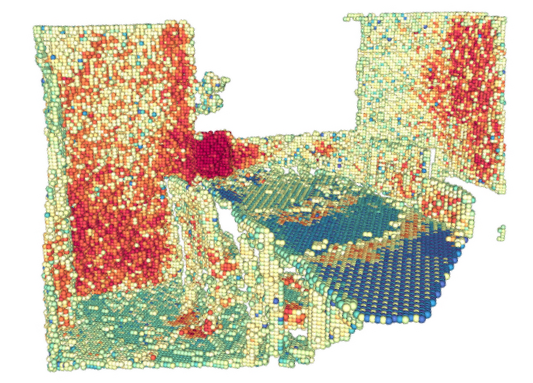
\includegraphics[width=4cm]{images/experiments/scratch-3d.png}
    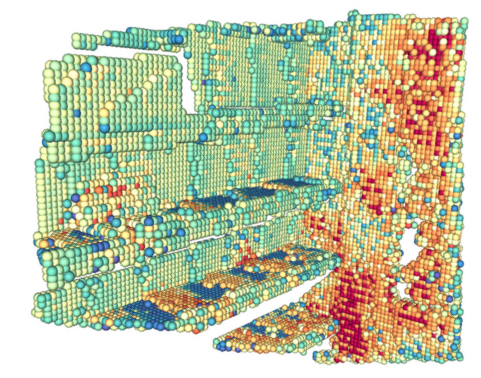
\includegraphics[width=4cm]{images/experiments/scratch-3d-2.png}
    \caption{Visualization of point features without pre-training.}
    \label{fig:features2dScratchvis}
\end{figure}

\subsection{Transfering 2D features to 3D}
\label{sec:results:2d3d}

To verify that the features were trasnfered correctly, we used the same visualization approach taken in section \ref{sec:results:2d} but instead applied it to points. Figure \ref{fig:features2d-3dvis} shows the relation between the 2D and 3D features. Although they didn't transfer perfectly, they did on certain key areas for example on the bookshelves in the top image and the wall and table in the lower image.

\subsection{Semantic Segmentation}
\label{sec:results:3d}

We first test the case of pretraining our model on ScannetV2 and finetuning on S3DIS. Our results are shown in table \ref{table:s3disResults}. Fully supervised pretraining has a drastic impact on the final downstream performance and is used as an upperbound on expected performance. Our algorithm is comparable to the performance of \cite{xie2020pointcontrast} however, that is without using overlapping 3D scans.

When using point correspondences without overlapping scans, the performance gain disappears almost entirely. This was noted in their original work and suggests to us that it is learning better features only due to its ability to better extrapolate surfaces.

Things to include in results
\begin{itemize}
    \item S3DIS semantic segmentation
    \item S3DIS instance segmentation
    \item Scannet semantic segmentation
    \item Scannet semantic segmentation with different amounts of data
    \item Visualization of features in 2D
    \item Visualization of features in 3D
    \item Pretraining and training without colour information
    \item Using projection of 3D points instead of direct scan using \cite{katz2007Direct}
    \item Training and validation curves
    \item Ablation studies
\end{itemize}

\section{Conclusion}
\label{sec:conclusion}



\newpage
%%%%%%%%% REFERENCES
{\small
    \bibliographystyle{ieee_fullname}
    \bibliography{contrastive-learning}
}

\end{document}